
\documentclass[10pt]{beamer}
\usepackage{times}
\usepackage{alltt}
\usepackage{proof}
\usepackage{tikz}

\input{dvipsnam.def}
\newenvironment{VampireProof}{%
	\section{Proof}}{}
\newenvironment{VampireInference}{%
	\begin{array}{c}}{\end{array}}
\newenvironment{VampireInferencePremises}{}{}
\newenvironment{VampirePremise}%
	{\begin{array}{l}}%
	{\end{array}}
\newenvironment{VampireConclusion}%
	{\begin{array}{l}}%
	{\end{array}}
\newcommand{\VampireUnit}[3]{%
	#1.~#2~[#3]}

\newcommand{\VPremiseSeparator}{\\}
%\newcommand{\VConclusionSeparator}{\\ \longrightarrow \\}
\newcommand{\VConclusionSeparator}{\\ \hline}

\newcommand{\Vor}{\vee}
\newcommand{\Vand}{\wedge}
\newcommand{\Vimp}{\supset}
\newcommand{\Viff}{\equiv}
\newcommand{\Vxor}{\not\equiv}

\newcommand{\VEmptyClause}{\Box}


\newcommand{\sLide}[1]{\begin{frame}\frametitle{#1}}

\AtBeginSection[]{\frame{\frametitle{Outline}\tableofcontents[current]}}

\setbeamercovered{dynamic}
\setbeamercolor{math text}{fg=MidnightBlue}

\definecolor{midnightblue}{cmyk}{0.98,0.13,0,0.43}
%\definecolor{olivegreen}{cmyk}{0.64,0,0.95,0.40}
\definecolor{rawsienna}{cmyk}{0,0.72,1,0.45}
\definecolor{fuchsia}{cmyk}{0.47,0.91,0,0.08}
\colorlet{redshaded}{red!25!bg}
\colorlet{shaded}{black!25!bg}
\colorlet{shadedshaded}{black!10!bg}
\colorlet{blackshaded}{black!40!bg}

\newcommand{\OliveGreen}[1]{{\color{OliveGreen}#1}}
\newcommand{\RedViolet}[1]{{\color{RedViolet}#1}}
\newcommand{\Mulberry}[1]{{\color{Mulberry}#1}}
\newcommand{\Fuchsia}[1]{{\color{Fuchsia}#1}}
\newcommand{\Brown}[1]{{\color{Brown}#1}}
\newcommand{\Black}[1]{{\color{Black}#1}}
\newcommand{\Magenta}[1]{{\color{Magenta}#1}}
\newcommand{\Green}[1]{{\color{Green}#1}}
\newcommand{\Purple}[1]{{\color{Purple}#1}}
\newcommand{\OrangeRed}[1]{{\color{OrangeRed}#1}}
\newcommand{\RoyalBlue}[1]{{\color{RoyalBlue}#1}}
\newcommand{\MidnightBlue}[1]{{\color{MidnightBlue}#1}}
\newcommand{\DarkOrchid}[1]{{\color{DarkOrchid}#1}}
\newcommand{\RedOrange}[1]{{\color{RedOrange}#1}}
\newcommand{\PineGreen}[1]{{\color{PineGreen}#1}}
\newcommand{\WildStrawberry}[1]{{\color{WildStrawberry}#1}}
\newcommand{\RawSienna}[1]{{\color{RawSienna}#1}}
\newcommand{\Periwinkle}[1]{{\color{Periwinkle}#1}}

\newcommand{\xone}[2]{{#1_{1},\ldots,#1_{#2}}}
\newcommand{\setof}[1]{{\{#1\}}}
\newcommand{\tuple}[1]{{\langle#1\rangle}}
\newcommand{\M}{}
\newcommand{\vs}{\visible}
\newcommand{\DI}[2]{\alert{#1}}
\newcommand{\DII}[3]{\alert{#1}}
\newcommand{\RR}{\Rightarrow}

%
%
% Algorithms
%
%

\newcommand{\inc}{~~~\= \+ \kill}    % used in algorithms
\newcommand{\dec}{\- \kill}         % used in algorithms

\newcommand{\reserved}[1]{\OliveGreen{\texttt{\bf #1}}}
\newcommand{\semicol}{\textbf{;}}                  % semicolon in algorithms
\newcommand{\commentinalg}[1]{\texttt{#1}}         % comment in algorithms
\newcommand{\PROCEDURE}{\reserved{procedure}}
\newcommand{\SUBPROCEDURE}{\reserved{subprocedure}}
\newcommand{\PARAMETERS}{\reserved{parameters}}
\newcommand{\INPUT}{\reserved{input}}
\newcommand{\LOOP}{\reserved{loop}}
\newcommand{\OUTPUT}{\reserved{output}}
\newcommand{\IF}{\reserved{if}}
\newcommand{\CASE}{\reserved{case}}
\newcommand{\OF}{\reserved{of}}
\newcommand{\DO}{\reserved{do}}
\newcommand{\OD}{\reserved{od}}
\newcommand{\THEN}{\reserved{then}}
\newcommand{\ELSE}{\reserved{else}}
\newcommand{\WHILE}{\reserved{while}}
\newcommand{\BEGIN}{\reserved{begin}}
\newcommand{\END}{\reserved{end}}
\newcommand{\LET}{\reserved{let}}
\newcommand{\FORALL}{\reserved{forall}}
\newcommand{\ASS}{\texttt{ := }}
\newcommand{\RETURN}{\reserved{return}}
\newcommand{\REPEAT}{\reserved{repeat}}
\newcommand{\VAR}{\reserved{var}}

\newcommand{\vampNot}{\~{}}    % negation in Vampire's output
\newcommand{\Active}{\mathit{active}}
\newcommand{\Given}{\mathit{given}}
\newcommand{\Unprocessed}{\mathit{unprocessed}}
\newcommand{\Passive}{\mathit{passive}}
\newcommand{\Current}{\mathit{current}}
\newcommand{\Init}{\mathit{init}}
\newcommand{\New}{\mathit{new}}
\newcommand{\Select}{\mathit{select}}
\newcommand{\Infer}{\mathit{infer}}
\newcommand{\Queue}{\mathit{queue}}
\newcommand{\Pop}{\mathit{pop}}
%\newcommand{\Mark}{\ding{52}}
\newcommand{\Mark}{\texttt{*}}
\newcommand{\Simplify}{\mathit{simplify}}
\newcommand{\Retained}{\mathit{retained}}
\newcommand{\ForwardSimplify}{\mathit{forward\_simplify}}
\newcommand{\Process}{\mathit{process}}
\newcommand{\BackwardSimplify}{\mathit{backward\_simplify}}
\newcommand{\GoalFound}{\mathit{goal\_found}}
\newcommand{\opt}[1]{\texttt{#1}}
\newcommand{\option}[1]{\opt{-#1}}
\newcommand{\Option}[1]{\opt{--#1}}
\newcommand{\optionval}[2]{\texttt{-#1~#2}}
\newcommand{\Optionval}[2]{\texttt{--#1~#2}}
\newcommand{\optionI}[1]{\texttt{-#1}\index{#1@\texttt{-#1}}}
\newcommand{\OptionI}[1]{\texttt{--#1}\index{#1@\texttt{--#1}}}
\newcommand{\optionvalI}[2]{\texttt{-#1~#2}\index{#1@\texttt{-#1}}}
\newcommand{\OptionvalI}[2]{\texttt{--#1~#2}\index{#1@\texttt{--#1}}}
\newcommand{\assign}{\texttt{:=}}                  % assignment in algorithms

%
% Multisets
%

\newcommand{\msminus}{\mathbin{\protect\dot{-}}} % multiset minus
\newcommand{\msin}{\mathbin{\protect\dot{\in}}}  % multiset membership
\newcommand{\msplus}{\mathbin{\protect\dot{+}}}  % multiset plues
\newcommand{\mscup}{\mathbin{\protect\dot{\cup}}}% multiset union
\newcommand{\mstimes}{\mathbin{\protect\dot{\times}}}% multiset product
\newcommand{\mscap}{\mathbin{\protect\dot{\cap}}}% multiset intersection
\newcommand{\mssubseteq}{\mathbin{\protect\dot{\subseteq}}} % sub multiset
\newcommand{\mssetof}[1]{{\protect\dot{\{}#1\protect\dot{\}}}} % multiset (explicit listing)
\newcommand{\mssetofb}{\protect\dot{\{}}     % multiset begin
\newcommand{\mssetofe}{\protect\dot{\}}}     % multiset end
\newcommand{\sizeof}[1]{|#1|}                % size of a multiset
                                % multiset-to-set conversion
\newcommand{\MtoS}[1]{\protect\stackrel{\curlywedge}{#1}}
                                % set-to-multiset conversion
\newcommand{\StoM}[1]{\protect\stackrel{\curlyvee}{#1}}

\newcommand{\eqbydef}{\stackrel{\text{def}}{=}}
\newcommand{\bydef}{\stackrel{\text{def}}{\Leftrightarrow}}

\newcommand{\rr}{\rightarrow}               % rewrite
\newcommand{\irr}{\leftarrow}               % inverse of rewrite
\newcommand{\nfrr}{\rr^!}                 % normal form rewrites
\newcommand{\nf}[1]{#1\downarrow}         % normal form binary relation

%
%
%   Logical notation
%
%
\newcommand{\imply}{\rightarrow}
\renewcommand{\implies}{\rightarrow}
\newcommand{\orl}{\vee}
\newcommand{\bigorl}{\bigvee}
\newcommand{\andl}{\wedge}
\newcommand{\bigandl}{\bigwedge}
\newcommand{\notl}{\neg}
\newcommand{\iffl}{\leftrightarrow}
\newcommand{\prov}{\vdash}
\newcommand{\Subst}[1]{\{#1\}}   % for substitutions
\newcommand{\subst}[2]{#1 \mapsto #2}   % for substitutions
\newcommand{\mgu}{\mathit{mgu}}
\newcommand{\mgs}{\mathit{mgs}}
\renewenvironment{proof}{
    {\em Proof.\/}}{
    \hfill $\Box${\vspace{4mm}}}
\newcommand{\true}{\mathrm{true}}
\newcommand{\false}{\mathrm{false}}
\newcommand{\intI}{I}                  % interpretation
\newcommand{\emptyclause}{\Box}

\newcommand{\ruleSup}{\mathsf{Sup}}
\newcommand{\ruleDem}{\mathsf{Dem}}
\newcommand{\ruleER}{\mathsf{ER}}
\newcommand{\ruleEF}{\mathsf{EF}}
\newcommand{\ruleFact}{\mathsf{Fact}}
\newcommand{\eql}{\simeq}
\newcommand{\neql}{\neq}
\newcommand{\deleted}[1]{#1}

%
%    Resolution
%

\newcommand{\mextension}[1]{#1^{\mathit{bag}}} % multiset extension of #1
\newcommand{\succm}{\mextension{\succ}}        % multiset extension of \succ
\newcommand{\succlm}{\mextension{\succl}}      % multiset extension of \succl
\newcommand{\succl}{\succ_{\mathit{lit}}}     % literal extension of \succ
\newcommand{\succeql}{\succeq_{\mathit{lit}}} % literal extension of \succ
\newcommand{\sel}{\sigma}                   % selection function
\newcommand{\BRr}{\mathsf{BR}}              % binary resolution rule
\newcommand{\Fact}{\mathsf{Fact}}           % factoring rule
\newcommand{\BRis}{\mathbb{BR}}             % binary resolution inference system
\newcommand{\SUPis}{\mathbb{SRF}}           % superposition inference system
\newcommand{\isI}{\mathbb{I}}               % inference system I
\newcommand{\sis}[1]{#1^{\mathrm{sat}}}     % saturating inference system bazed on I
\newcommand{\BRiss}{\mathbb{BR}_{\sel}}     % binary resolution inference system with selection
\newcommand{\SUPiss}{\mathbb{S}\mathrm{up}_{\succ,\sel}}   % SUPis with selection
\newcommand{\TA}{\mathit{TA}}               % term algebra
\newcommand{\nat}{\mathbb{N}}               % natural numbers
\newcommand{\KBo}{\succ_{\mathit{KB}}}   % Knuth-Bendix ordering
\newcommand{\wf}{w}               % weight function
\newcommand{\weight}[1]{|#1|}     % weight of term


\colorlet{darkred}{red!80!black}
\colorlet{darkblue}{blue!80!black}
\colorlet{darkgreen}{green!80!black}
\colorlet{darkergreen}{green!60!black}

\def\radius{0.96cm}
\def\innerradius{0.85cm}

\def\softness{0.4}
\definecolor{softred}{rgb}{1,\softness,\softness}
\definecolor{softgreen}{rgb}{\softness,1,\softness}
\definecolor{softblue}{rgb}{\softness,\softness,1}

\definecolor{softrg}{rgb}{1,1,\softness}
\definecolor{softrb}{rgb}{1,\softness,1}
\definecolor{softgb}{rgb}{\softness,1,1}

\author{
  \textcolor{red!90!black}{Laura Kov\'acs}}
\titlegraphic{\hspace*{1em}
\includegraphics[width=.5\textwidth]{forsyte}}

\newcommand{\Blue}[1]{{\color{blue}#1}}

%
% Misc
%
\newcommand{\clr}[2]{\mathit{\OliveGreen{#1}\Red{#2}}}

\title{
              	       Automated Deduction
}

%
%
\author{
  \textcolor{red!90!black}{Laura Kov\'acs} \\
\titlegraphic{\hspace*{1em}
\includegraphics{forsyte}}}
\begin{document}

\date{}
\frame{\titlepage}




%---------------------------------------------------------------------

\section{First-Order Theorem Proving - An Example}
%\section{Introduction}

\begin{frame}
\frametitle{First-Order Theorem Proving}

We will use the {\sc Vampire} theorem prover throughout the lecture. \\[1em]

\onslide<2->{
Go to
\begin{center}
\url{https://vprover.github.io/download.html}
\end{center}
and pick the route most suitable to you.

\vspace{1em}\noindent
Note:
          \begin{itemize}
          \item only running Vampire in the browser at
   \\
\url{https://tptp.org/cgi-bin/SystemOnTPTP}
            \end{itemize}
}
\end{frame}



%---------------------------------------------------------------------

\subsection{First-Order Logic and TPTP}

\input{intro_tptp}
%---------------------------------------------------------------------

\subsection{Running a First--Order Prover}

%-----------------------------------------------------
                                

\begin{frame}
\frametitle{Running Vampire on a TPTP file}

is easy: simply use

\Blue{%
\begin{alltt}
vampire <filename>
\end{alltt}}

\bigskip

\vs<2->{
One can also run Vampire with various options, some of them will be
explained later. For example, save the group theory problem in a file
\texttt{group.tptp} and try 

\Blue{%
\begin{alltt}
vampire --thanks ADuct25 group.tptp
\end{alltt}}
}

                  \end{frame}


%---------------------------------------------------------------------

\begin{frame}
  \frametitle{Proof by Vampire (Slightly Modified)}

\vspace*{-2ex}

\footnotesize
\begin{alltt}
\hskip-3em\alert<7>{Refutation found}.\\*[-0.7ex]
\hskip-3em\alert<6,7>{\alert<9>{251}. \$false [{\color<8>{blue}trivial inequality removal} 250]}\\*[-0.7ex]
\hskip-3em\alert<6>{\alert<9>{250}. mult(sk0,sk1) != mult (sk0,sk1) [{\alert<8>{superposition}} 14,159]}\\*[-0.7ex]
\hskip-3em\alert<6>{\alert<9>{159}. mult(X0,X1) = mult(X1,X0) [\alert<8>{superposition} 23,87]}\\*[-0.7ex]
\hskip-3em\alert<6>{\alert<9>{87}. mult(X1,mult(X0,X1)) = X0
  [{\color<8>{blue}forward demodulation} 79,25]}\\*[-0.7ex]
\hskip-3em\alert<6>{\alert<9>{79}. mult(X1,mult(X0,X1)) = mult(X0,e) [\alert<8>{superposition} 23,20]}\\*[-0.7ex]
\hskip-3em\alert<2,6>{\alert<9>{25}. mult(X0,e) = X0 [\alert<8>{superposition} 23,13]}\\*[-0.7ex]
\hskip-3em\alert<2,6>{\alert<9>{23}. mult(X0,mult(X0,X1)) = X1 [{\color<8>{blue}forward demodulation} 15,10]}\\*[-0.7ex]
\hskip-3em\alert<6>{\alert<9>{20}. e = mult(X0,mult(X1,mult(X0,X1)))  [\alert<8>{superposition} 13,12]}\\*[-0.7ex]
\hskip-3em\alert<6>{\alert<9>{15}. mult(X0,mult(X0,X1))=mult(e,X1)  [\alert<8>{superposition} 12,13]}\\*[-0.7ex]
\hskip-3em\alert<4>{\alert<9>{14}. mult(sK0,sK1) != mult(sK1,sK0) [cnf transformation 9]}\\*[-0.7ex]
\hskip-3em\alert<4>{\alert<9>{13}. e = mult(X0,X0) [cnf transformation 4]}\\*[-0.7ex]
\hskip-3em\alert<4>{\alert<9>{12}. mult(X0,mult(X1,X2)) = mult(mult(X0,X1),X2) [cnf transformation 3]}\\*[-0.7ex]
\hskip-3em\alert<4>{\alert<9>{10}. mult(e,X0) = X0 [cnf transformation 1]}\\*[-0.7ex]
\hskip-3em\alert<2,4,5>{\alert<9>{9}. mult(sK0,sK1) != mult(sK1,sK0) [skolemisation 7,8]}\\*[-0.7ex]
\hskip-3em \alert<4,5>{\alert<9>{8}. ?[X0,X1]: mult(X0,X1) != mult(X1,X0) <=> mult(sK0,sK1) != mult(sK1,sK0) \\
\hskip33em[choice axiom]}\\*[-0.7ex]
\hskip-3em\alert<4>{\alert<9>{7}. ?[X0,X1]: mult(X0,X1) != mult(X1,X0) [ennf transformation 6]}\\*[-0.7ex]
\hskip-3em\alert<4,7>{\alert<9>{6}. \vampNot![X0,X1]: mult(X0,X1) = mult(X1,X0) [negated conjecture 5]}\\*[-0.7ex]
\hskip-3em\alert<3>{\alert<9>{5}. ![X0,X1]: mult(X0,X1) = mult(X1,X0) [input(conjecture)]}\\*[-0.7ex]
\hskip-3em\alert<3>{\alert<9>{4}. ![X0]: e = mult(X0,X0)[input(assumption)]}\\*[-0.7ex]
\hskip-3em\alert<3>{\alert<9>{3}. ![X0,X1,X2]: mult(X0,mult(X1,X2)) = mult(mult(X0,X1),X2) [input(axiom)]}\\*[-0.7ex]
%\hskip-3em\alert<3>{\alert<9>{2}. ![X0]: e = mult(inverse(X0),X0) [input]}\\*[-0.7ex]
\hskip-3em\alert<3>{\alert<9>{1}. ![X0]: mult(e,X0) = X0 [input(axiom)]}\\*[-0.7ex]
\end{alltt}

%\vspace*{-3ex}


\begin{itemize}
\item \vs<2->{\alert<2>{Each inference derives a formula from zero or more other formulas;}}
\item \vs<3->{\alert<3>{Input}, \alert<4>{preprocessing},
    \alert<5>{new symbols introduction}, \alert<6>{superposition 
  calculus}}
\item \vs<7->{\alert<7>{Proof by refutation}, \alert<8>{generating}
    and
    {\color<8>{blue}simplifying} inferences,
  \alert<9>{unused formulas} \ldots}
\end{itemize}

                                \end{frame}

%---------------------------------------------------------------------



                                
                      \begin{frame}
                 \frametitle{Vampire}


\begin{itemize}
\item \alert{Completely automatic:} once you started a proof attempt,
  it can only be interrupted by terminating the process.\\[1em]


\item \visible<2->{\alert{Champion} of the CASC world-cup  in
    first-order theorem proving: won CASC $>$ 70
  times. \\[.5em]


  \begin{center}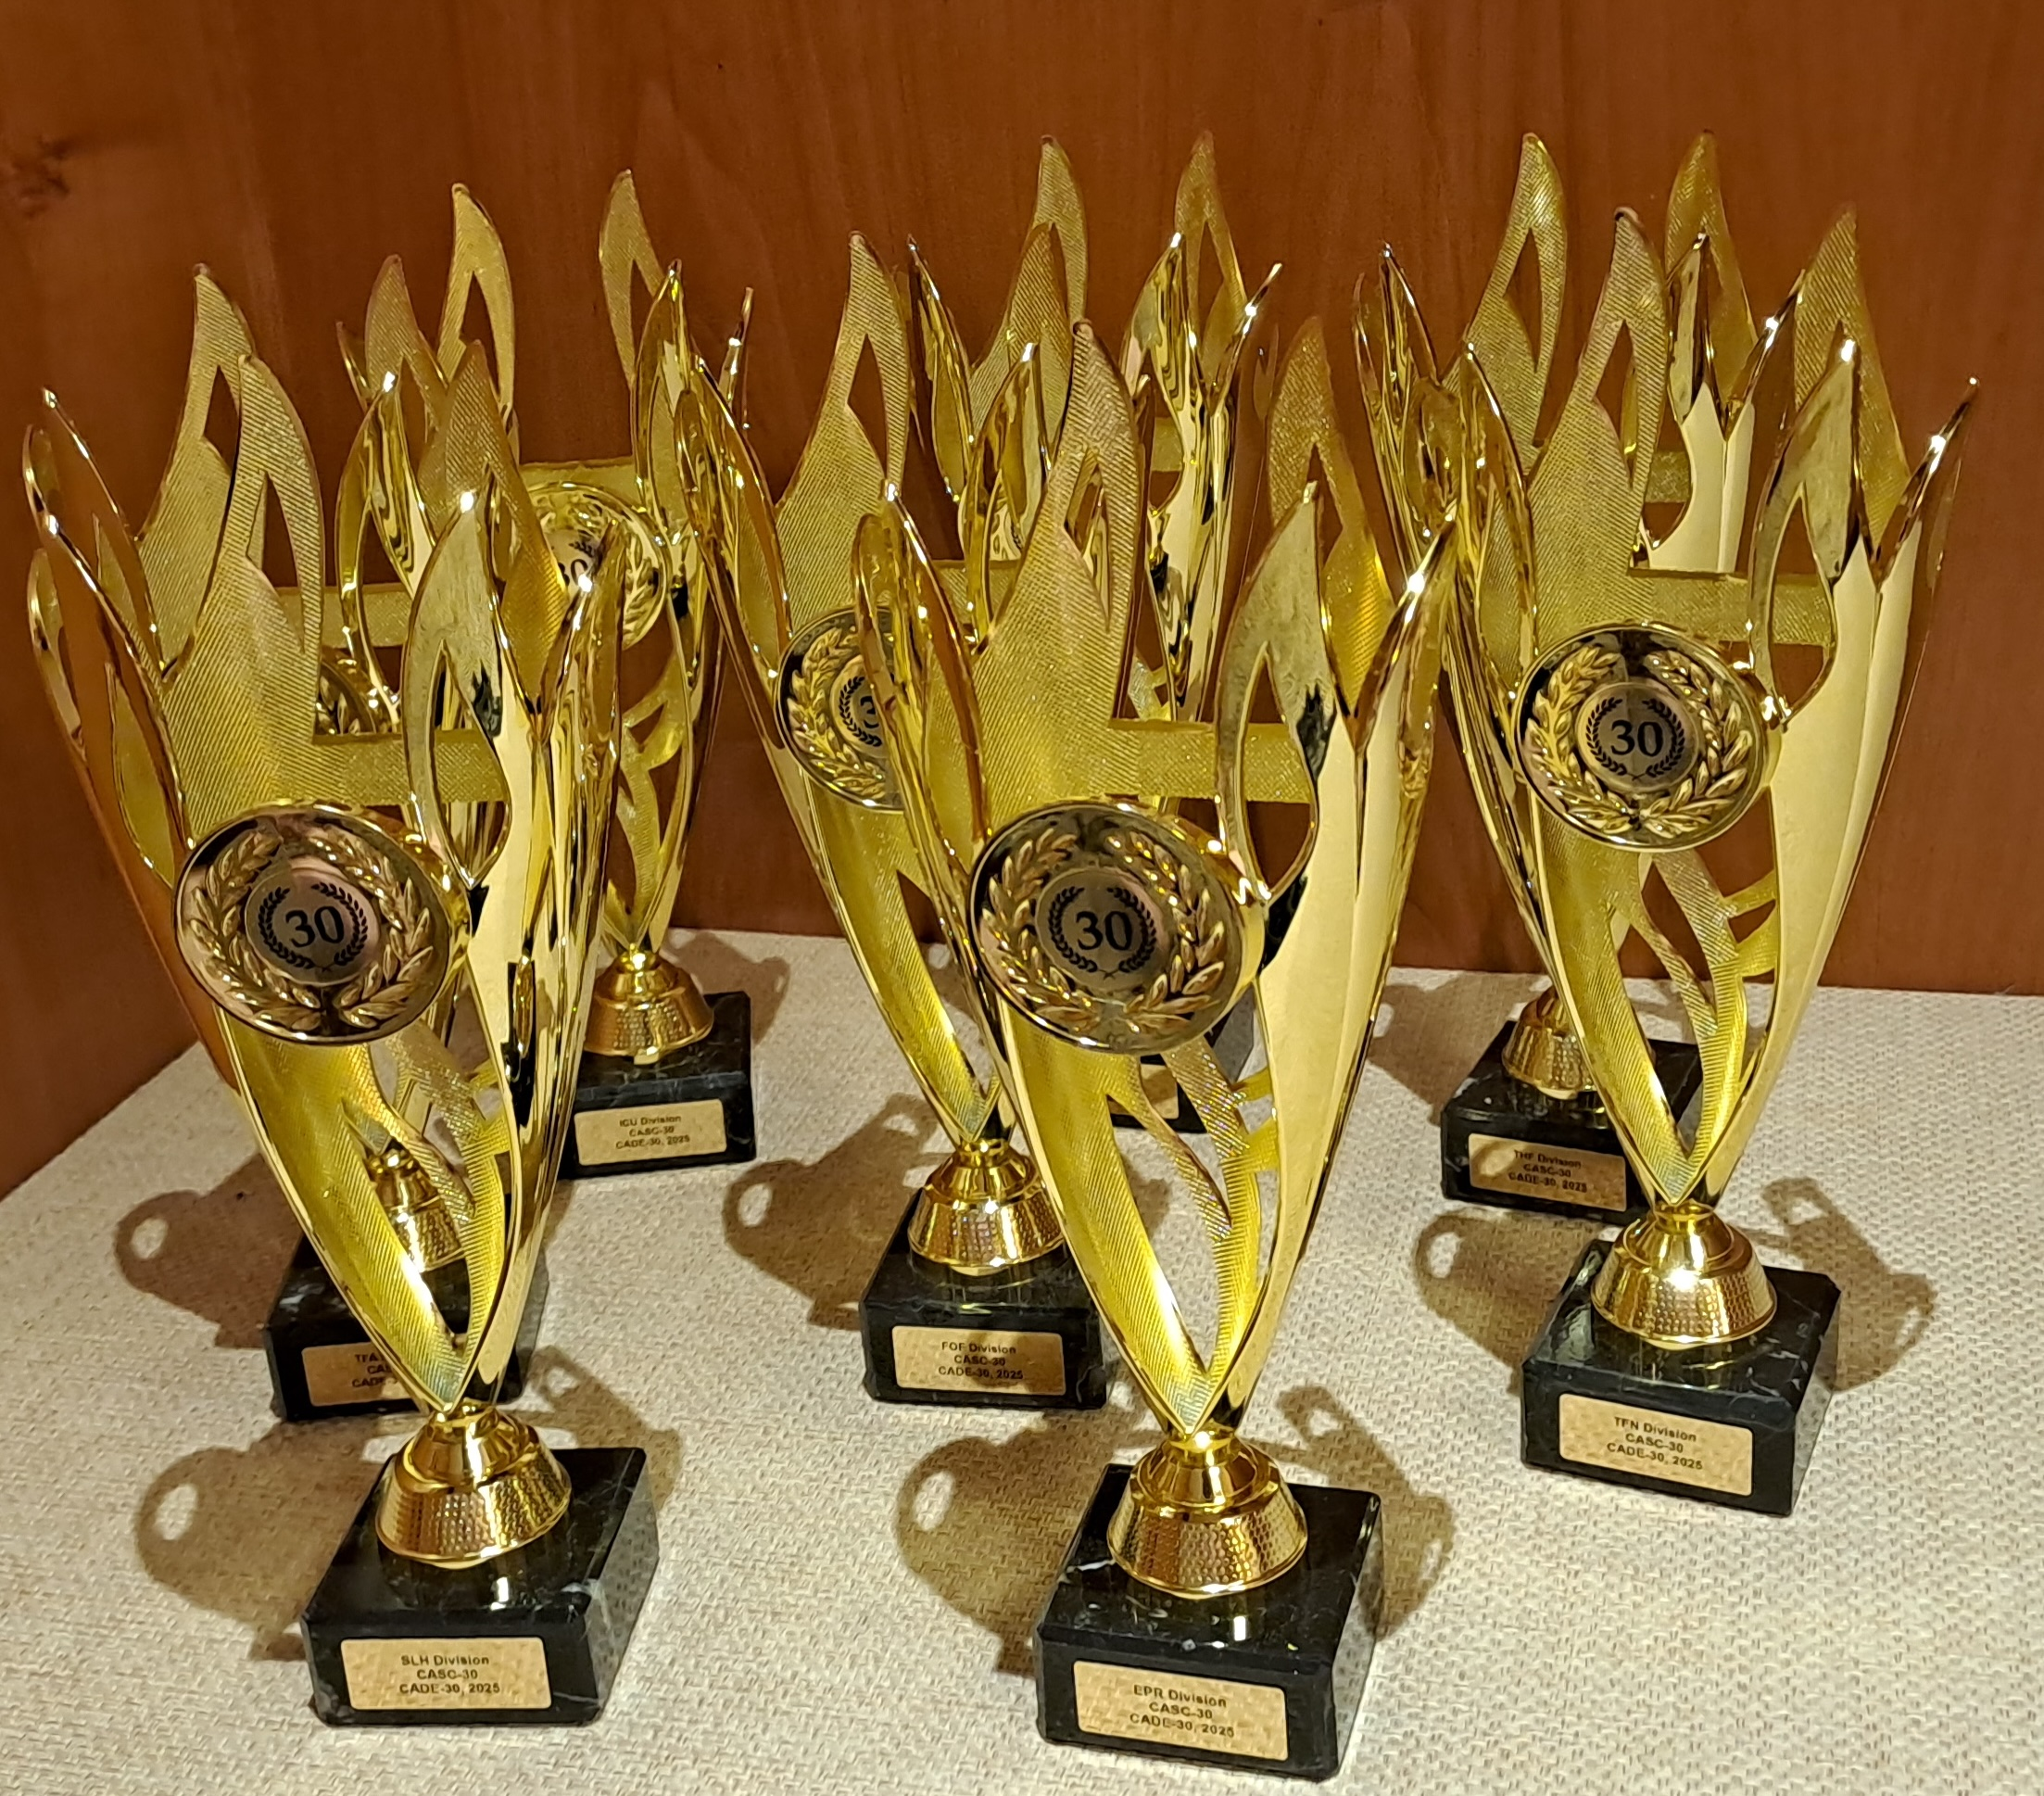
\includegraphics[scale=.07]{Vampire5_CASC.jpg}\end{center}


}
\end{itemize}

                               \end{frame}

                               
%---------------------------------------------------------------------
                                
                      \begin{frame}
                 \frametitle{Vampire - The Team at CASC 2025}
\begin{center}
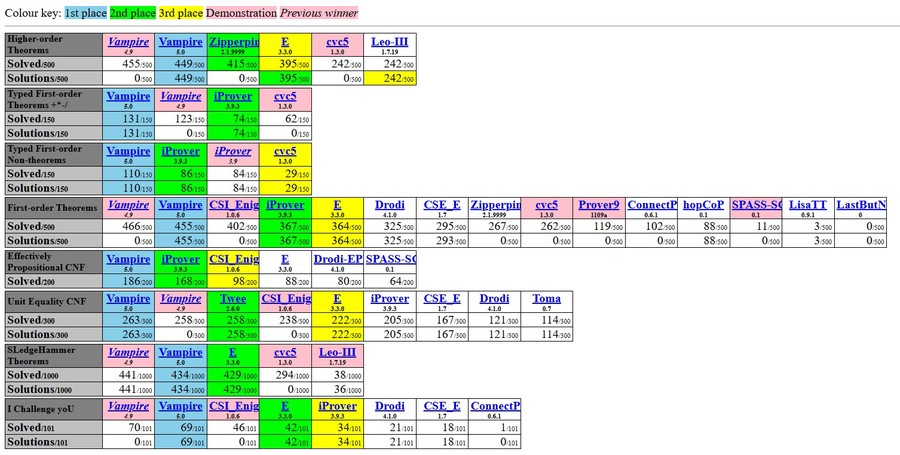
\includegraphics[scale=.5]{casc25.jpg}
\end{center}

\end{frame}
                 
%---------------------------------------------------------------------



                               
                                
                      \begin{frame}
                        \frametitle{Vampire - The Team at CAV 2025}

                        \begin{center}
                          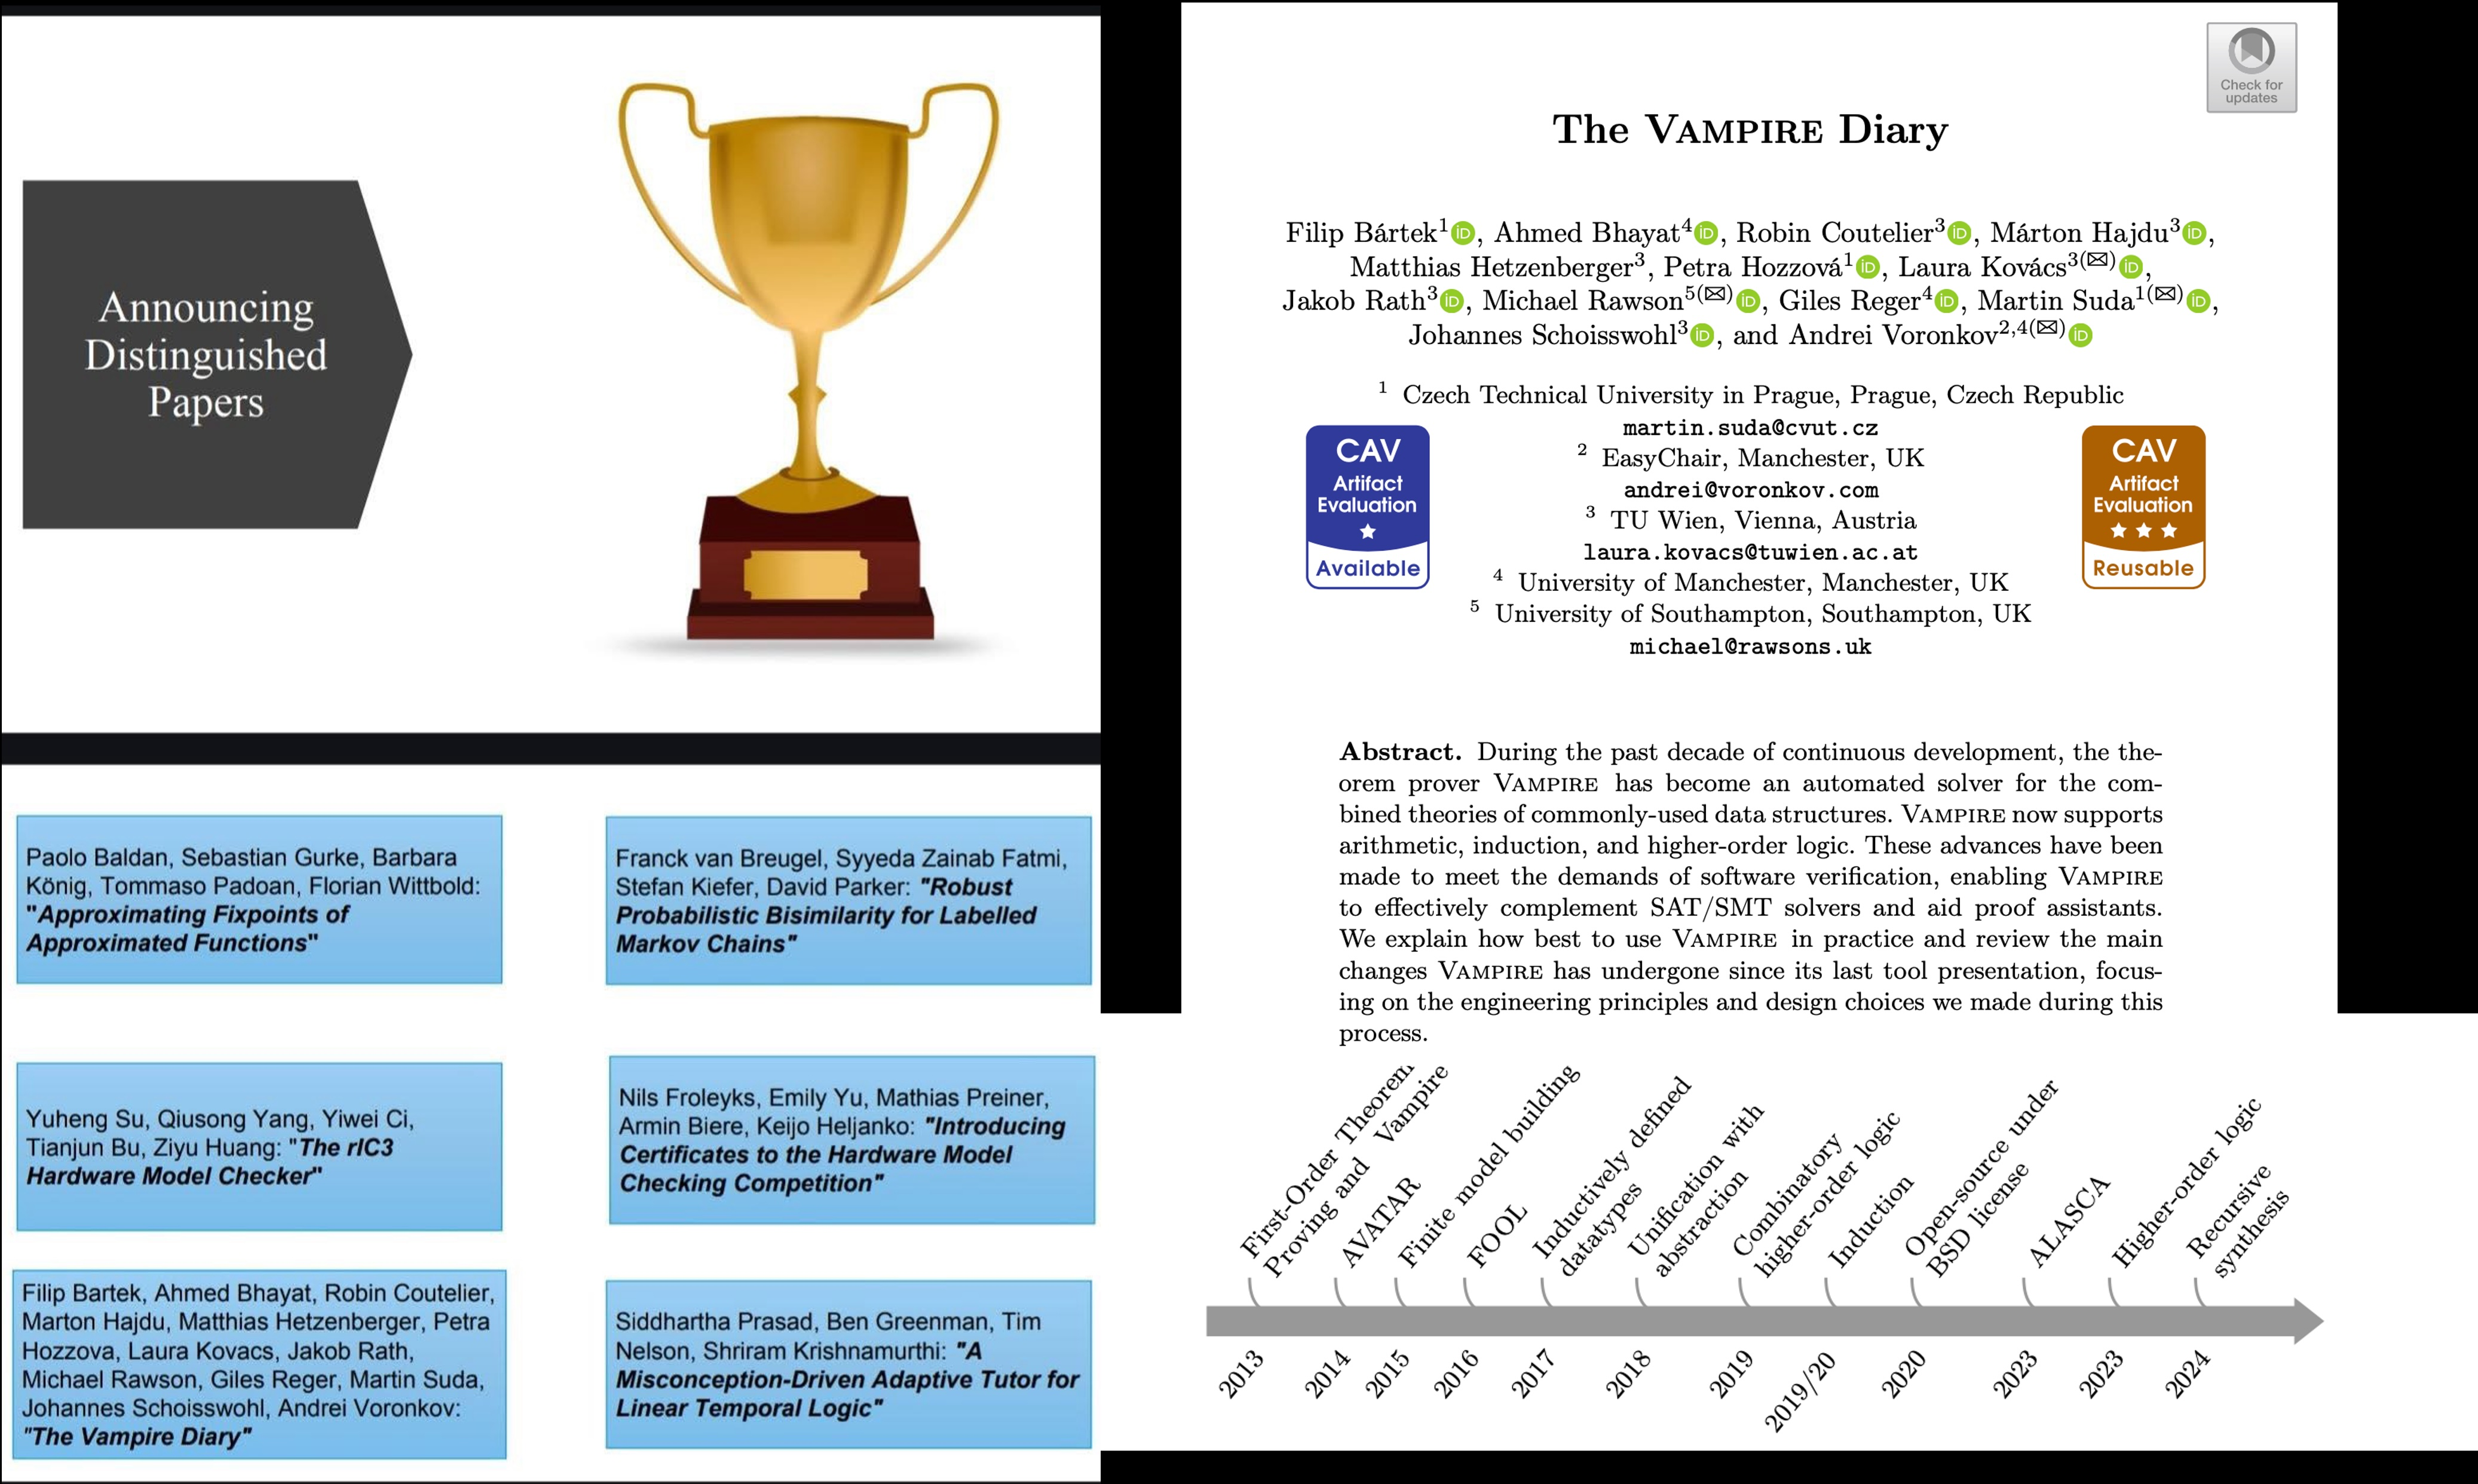
\includegraphics[scale=.35]{Vampire_CAV25.jpg}
                          \end{center}

                        
                        \end{frame}


        %---------------------------------------------------------------------

                             
%---------------------------------------------------------------------



\end{document}


